\section{\projectname{}}
\label{sec:metalloc}

As we have seen, one of the major limitations of state-of-the-art
memory shadowing approaches is the difficulty of getting the compression ratio right.
Because the right value may differ from application to application, the
intuitive solution is to enable a variable compression ratio.
This eliminates the fixed memory overhead associated with metadata shadowing
and greatly reduces the allocation-time performance hit.
%It also introduces the need for an additional mechanism to infer the appropriate compression ratio
%during metadata retrieval.
\begin{comment}
This scheme is used in the sanitizer library of LLVM as a means to track metadata
with manageable memory overhead. 
It groups most heap allocations into regions based on their size, with each region organizing objects
into buckets of a unique size. Intuitively each region is associated on the largest possible compression ratio,
mapping each bucket to one piece of metadata. Lee et al.~\cite{lee2015type} showcase it as
effective for checking the type safety of cast operations at run time, but they also 
highlight some limitations, such as the inability to use this metadata tracking system
for global and stack objects. The allocator also lacks address randomization and
the ability to reclaim physical memory, making it unsuitable
for general purpose deployment.\EK{we are no longer presenting this ibn this paper; should we bring it back?}
% For an arena-based system this
% is equivalent to identifying the arena which owns the pointer itself. This
% process has not yet been designed with performance in mind within the LLVM implementation.
\end{comment}

\projectname{}'s key goal is to implement a metadata management scheme
handling all memory objects in a uniform and highly efficient manner, regardless of
their allocation type (heap, stack, or global memory).
There are two requirements 
to accomplish this goal.
The first is to support a simple, efficient, and uniform mechanism
to associate pointers with the compression ratio. The second is the
ability to optimize the compression ratio as much as possible, ideally such that only a single
metadata is needed for each object. \projectname{} meets both these requirements
by ensuring that all the memory objects within a memory page can be
associated with a nontrivial common alignment, which does not change
as long as there are active objects within the page. 
This requirement serves as a basis for our scheme and is met
by drawing from modern heap~\cite{ghemawat2009tcmalloc} and stack~\cite{kuznetsov2014cpi} organizations
widely used in production, as discussed in Section~\ref{sec:assumptions}.

Alignment relates directly to the compression ratio, namely an $n$-byte object
alignment allows one \emph{metadata entry} to be associated to every group of $n$ bytes
within said object. Having uniform alignment within each memory page allows 
\projectname{} to associate compression ratios to the individual memory
pages and to look them up using a mechanism similar to \emph{page tables}. Such page tables
also include the location of the metadata region corresponding to the individual pages.
This mechanism is described in the following section.

\subsection{Efficient retrieval of page information}
\label{sec:pageinfo}

Because lookups are expected to be very frequent, the page table design is very
performance-sensitive. For this reason, \projectname{} opts for a single-level page table design,
which requires only one memory read for each lookup. We refer to this data structure as the
\emph{meta-page table}. 
Figure~\ref{fig:metalloc} shows the general operating principle of \projectname{},
including the use of the meta-page table.
Given a pointer, we spit it in a page index and an offset.
The page index is used as an index into the meta-page table,
which is an array stored at the page table base.
This page table base is a compile-time constant and therefore requires no extra memory read.
The entries in this array are eight bytes large, split between the seven-byte \emph{metabase} pointer and
the one-byte base-2 logarithm of the memory alignment.
The metabase points to the start of an array of metadata entries
available for this page table entry.
The size of the entries of the metadata array is determined by the \emph{metasize}
compile-time constant, which specifies the amount of metadata per object.
It should be noted that objects larger than the alignment size have multiple
metadata entries, each with the same contents.
The offset part of the original pointer divided by the alignment serves
as an index into the metadata array, allowing the correct metadata entry to be
located for the specified object.

\begin{figure}[t]
\center
  \includegraphics[width=3.5in]{figs/metalloc.pdf}
  \caption{
  \projectname{}'s metadata lookup
  }
  \label{fig:metalloc}
  \vspace{-1em}
\end{figure}

While the size of the meta-page table (for x86-64 systems using 48-bit virtual addresses and 4096-byte pages)
is theoretically $2^{36}$ entries or $512$ GB, only the parts corresponding to address ranges currently in use by the process need to be allocated. To implement this strategy, \projectname{} reserves the required virtual memory area in advance and relies on demand paging to lazily link the required page table pages to physical memory.
\begin{comment}
A backup mechanism
is necessary to stop the continuous expansion of the meta-page table as the program potentially
migrates its data from one virtual address range to another during execution (for address randomization for instance).
\end{comment}

\begin{comment}
We solve this problem by including a secondary ref-count table which tracks the usage of the meta-page table.
Whenever we detect that a virtual page within the meta-page table becomes unused by the process, we notify the
OS to release the underlying physical storage. The ref-count table only needs a two-byte counter for 
each virtual page of the meta-page table, limiting its size to
$2^{27}$ entries or $256$ MB of virtual memory. This can be further reduced
by grouping multiple pages in the same entry. The ref-count table is accessed and manipulated only during \texttt{mmap}
and \texttt{munmap} operations (when the virtual address range of the process changes),
thus it does not affect the critical path of the program.
\IH{don't we jut take out the hit-count table for EuroSec and mention it briefly?}
\end{comment}

\subsection{Static versus dynamic metadata}
\label{sec:metadata}

The scheme presented so far assumes a fixed-sized metadata entry
which is statically initialized at the start of the object's lifetime.
For objects whose size exceeds their alignment there are multiple copies
of this metadata entry in memory.
A metadata entry can be an integer, a small struct
or even a pointer, which can refer to further metadata of arbitrary dynamic size.

\CRI{We always talk about amount of metadata to refer to both ``sizeof(user-metadata)'' and ``sizeof(user-metadata)*copies''. We need make a clear distinction between the two in the paper, or readers will be lost. For instance, the term ``metadata node'' appears out of the blue below, while it should appear much earlier.}\IH{I introduced the term metadata node in the previous section and tried to eliminate confusing terminology, is it better now?}
In the simplest possible setup, each metadata entry is filled with a compile-time constant,
such as a type index. This scheme allows the instrumentation to identify certain predetermined object characteristics at run time, with the lowest possible overhead. In this use case, initializing the
metadata is cheap, as it involves a simple \texttt{memset} operation for the compressed metadata range corresponding to the object. Given the use of variable compression rates, the amount of metadata that needs to be initialized is minimal.

Alternatively, the metadata can include a pointer to information created
at compile time in global memory. This scheme may be, for example, used to
support in-depth type tracking when implementing precise garbage collection
for languages such as C/C++~\cite{rafkind2009precise}.
From an overhead perspective, this is similar to the constant metadata scenario, as the pointer itself is just another numeric constant,
% (or a PC-relative value)
whose value is fixed at compile time.

Finally, the metadata pointer might be generated at run time.
In this case, a \emph{metadata node} is allocated whenever a new memory object
is allocated and deallocated when the memory object is. 
This scheme is relevant to instrumentation tailored to individual object
instances, rather than broad object groups. Sharing lifetimes is trivial on the
stack and in global memory, but leads to interesting design decisions when dealing
with the heap. Intuitively, the fastest solution is to increase the allocated size
of the object itself and store the metadata node in-band. In practice, we found
this solution to result in significant performance degradation due to its
negative  impact on caching.
The alternative is to perform a second heap allocation dedicated to the metadata node 
itself. While we expected a nontrivial performance hit for applications where allocations
dominate the run time, we found the impact to be reasonable in practice.
% We suspect that
% this is made possible by the efficiency of tcmalloc when allocating from a homogeneous
% pool of fixed-sized objects.
In addition, most applications do not require object-specific metadata tracking
and can safely refrain from using dynamic metadata (which incurs the highest run-time and memory overhead).
\CRI{We don't discuss metadata integrity at all here. This may be fine for EuroSec if we don't have any story at all, but I suspect the solution to have both performance and integrity is to allocate the deep metadata node right after the first pointer copy (forcing a larger minimum alignment).}\IH{Not alignment per-se, but you force each metadata node to be significantly larger.}

\subsection{Instrumentation across memory types}
\label{sec:assumptions}

\textbf{Globals}. Global memory is the simplest to deal with from a memory shadowing perspective. Global allocations only occur at load time and the amount of global data is typically
limited. These properties suggest that the default 8-byte alignment within the system works reasonably well for this allocation type, thus we can just associate every global data memory page with this alignment in the meta-page table.
We simply instrument binary files (executables and dynamic libraries) to allocate metadata pages and set up the meta-page table entries corresponding to their data sections as soon as the binaries are loaded.

\textbf{Stack}. Stack pages share the property of long lifetimes with global memory (associated with the stack for the lifetime of the thread), but they are unique in that object allocations within the pages occur frequently and with minimal run-time cost. A simple solution is to restrict stack objects to the conservative 8-byte alignment~\cite{akritidis2008preventing},
% since the stack also includes a number of spilled registers or ABI specified elements
% which have restricted movement.
but this makes tracking multi-byte metadata
prohibitively expensive. \projectname{} solves this challenge by leveraging recent advances
in shadow stack solutions (recently integrated in mainstream compilers)~\cite{kuznetsov2014cpi}, which split the program stack into a primary and a secondary stack.
We propose using a multi-stack approach with a primary and a number of secondary stacks. The primary stack would preserve all the stack objects not subject to
the current instrumentation, including ABI specific elements such as return addresses and arguments. Objects subjected to instrumentation are moved to one of the secondary
stacks based on their size. This design ensures that \projectname{} only needs to care about the secondary stacks, which are free from ABI specific restrictions.
In practice we propose using the same heuristic for all instrumentations, namely moving all objects which can potentially be subject to memory
corruption attacks (either address taken or address used in unpredictable manner) to one of the secondary stacks. In general the secondary stacks end up composed
mostly of arrays and some address taken integers. As a result we propose enforcing a fixed but
large alignment on each object within every secondary stacks. While some memory fragmentation
does occur with address taken integers, it only affects a small portion of the entire
memory address space of the program and it will not break program functionality in general.
Our current design uses one secondary stack for small and medium objects having a fixed alignment of 64 bytes,
and another secondary stack for large objects where 4096 byte alignment is enforced.
\projectname{} instruments the allocation of program stacks to create the secondary stacks
and to also allocate the corresponding metadata pages and to set up the appropriate meta-page table entries.

\CRI{As above, we need to make this design section self-contained and not using oblivious writing (i.e., we're like X except plus Y and minus Z). We can say we draw from recent allocator design (tcmallocREF) to organize the heap as X, Y, Z to match our assumptions (as above), but then we have to explain things end-to-end and forget about tcmalloc here. We can just have the next (short) subsection named Implementation, which mentions ``We implemented METAlloc in etc. etc. For stack management, we modified SafeStack to do X. For heap management, we modified tcmalloc to do Y.}
\textbf{Heap}.
In order to meet our requirements, we propose a heap allocator designed around the concept of object sizes.
Instead of keeping track of the heap as a whole, it operates with size-specific free-lists instead.
Whenever a free-list becomes empty, the allocator can request new memory pages from the system, which are
then associated with this particular free-list until they are released back to the system. The allocator would then
enforce the largest possible alignment for objects within each free-list wiithout triggering too much
fragmentation. Applying \projectname{} to such a heap allocator is trivial as one just needs to monitor
page request by the free-lists to associate the appropriate metadata information with the pages. Figure~\ref{fig:metalloc-heap}
summarizes this operation with the addition of potential object caches and a page allocator to improve performance.

\subsection{Implementation specifics}
\label{sec:assumptions}

While it is possible to build a brand new custom heap allocator which respects our design specification
, we decided to build upon a proven, state-of-the-art allocator instead. We expect that for most
complex C++ applications the heap allocator has a significant impact
on performance, thus a proven allocator is key. The tcmalloc allocator 
(developed and used by Google) features a memory organization which matches up well with our design.

For the stack we decided to extend the implementation of SafeStack~\cite{kuznetsov2014cpi}, as it is advertised
as a replacement for stack canaries going forward and it is becoming a core component within the LLVM
project. Its interpretation of safe and unsafe objects also matches up well with our definition of objects
requiring instrumentation. 

\begin{comment}Its central free list operates on the basis of memory spans. Each span is a set of contiguous memory pages
configured to include a specific class of objects defined by their size. These spans
are allocated and deallocated monolithically, the central free list not having
control over the span configuration. The allocator ensures the same alignment 
(as large as possible, while restricting fragmentation) for all the objects 
within a span. We extend tcmalloc by allocating metadata pages and updating
the meta-page table whenever a new span is allocated. Figure~\ref{fig:metalloc-heap}
summarizes this operation.\end{comment}

\begin{figure}[t]
\center
  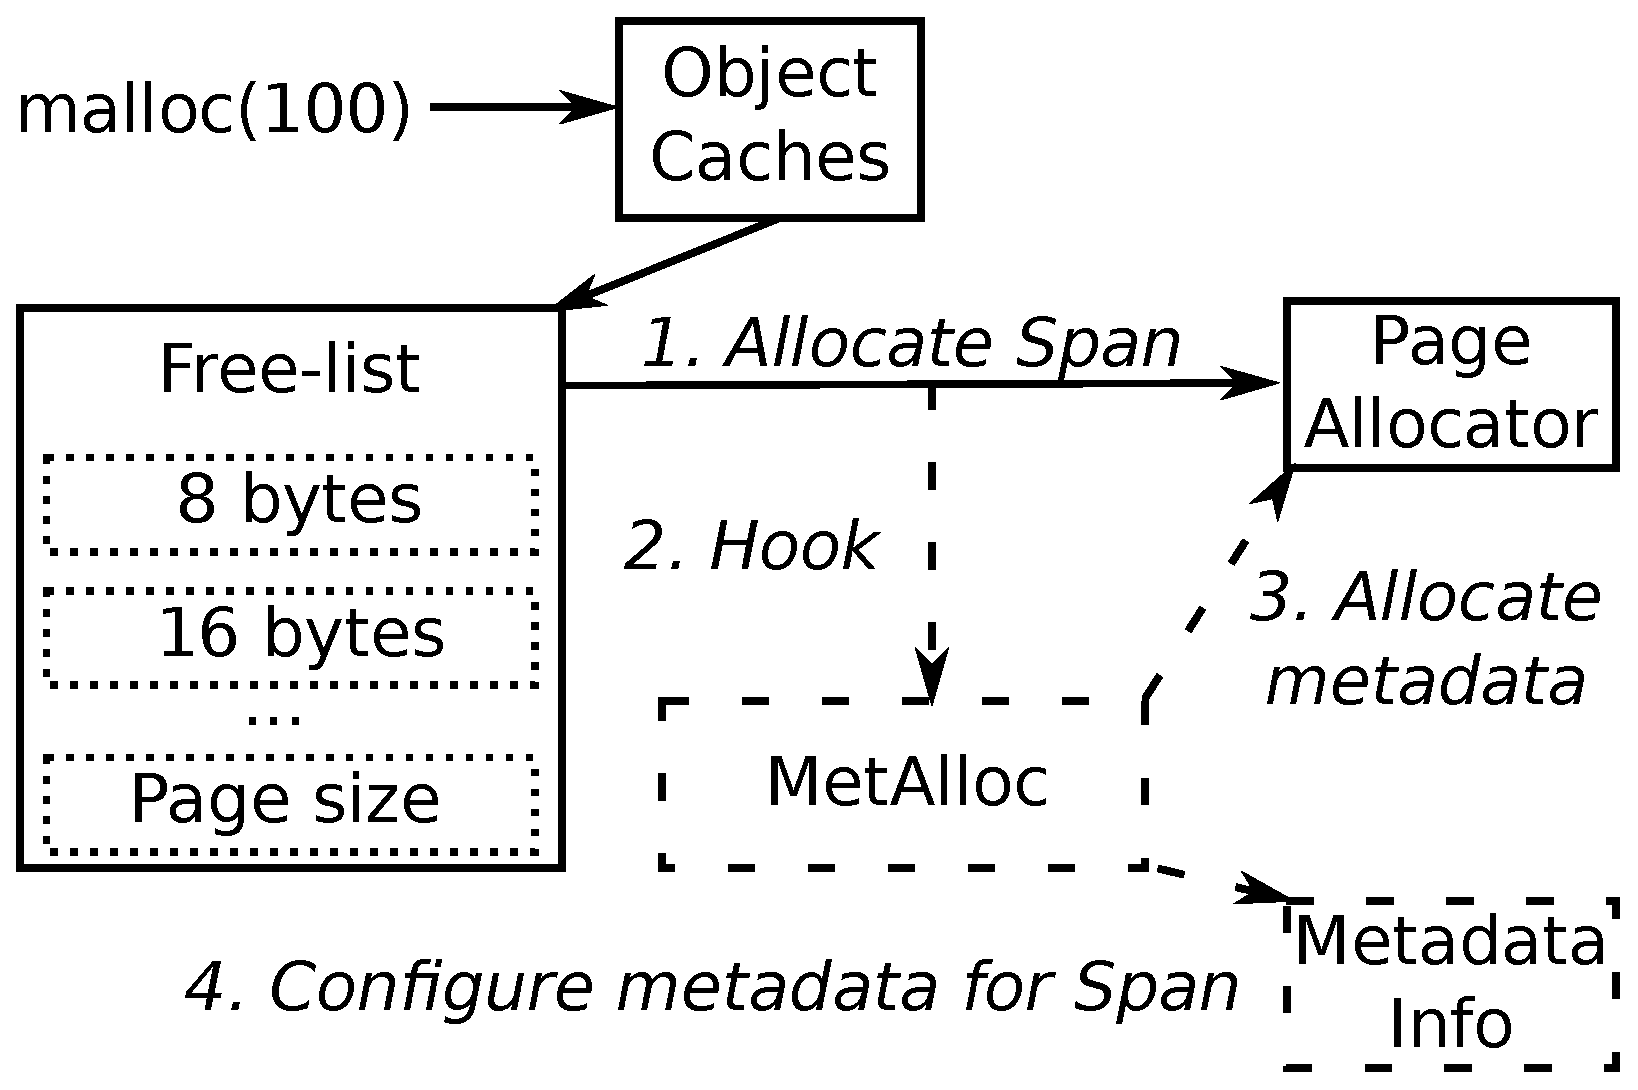
\includegraphics[width=2.8in]{figs/metalloc-heap.eps}
  \caption{
  Heap metadata management using \projectname{}
  }
  \label{fig:metalloc-heap}
  \vspace{-1em}
\end{figure}


